\chapter{Hito 4: Despliegue y operacionalizaci\'on del sistema}
\label{chap:hito4}

\section{Introducci\'on}

El cuarto hito del proyecto tiene como objetivo transformar el trabajo experimental realizado en los hitos anteriores
en un sistema desplegable, reproducible y orientado a su uso operativo. Para ello, se ha dise\~nado una soluci\'on basada
en contenedores que separa las fases de entrenamiento e inferencia.

En este hito se ha estructurado el proyecto en componentes independientes y configurables. Esta decisi\'on permite encapsular 
dependencias, reducir problemas de portabilidad y acercar el sistema a un escenario real de despliegue.

Adem\'as del propio despliegue, este cap\'itulo pone el foco en las decisiones de dise\~no adoptadas para dividir el sistema
en m\'odulos Python y contenedores diferenciados. Se justifica por qu\'e se ha optado por esta estructura y se analizan las
implicaciones t\'ecnicas que ha tenido sobre el desarrollo, la ejecuci\'on y la mantenibilidad del proyecto.

\section{Arquitectura general del despliegue}

La arquitectura implementada se compone de dos servicios principales: un contenedor de entrenamiento y un contenedor de inferencia.
El primero se encarga de entrenar el modelo a partir del conjunto de datos del proyecto y almacenar el artefacto resultante; el segundo
carga dicho modelo y expone una API web para realizar predicciones desde el exterior.

A nivel de repositorio, la l\'ogica de entrenamiento e inferencia se ha desacoplado en los archivos \texttt{src/train.py} y \texttt{src/infer.py}.
Adem\'as, la construcci\'on de cada servicio se ha separado en los archivos \texttt{Dockerfile.train} y \texttt{Dockerfile.infer}, mientras que
la orquestaci\'on conjunta se realiza mediante \texttt{docker-compose.yaml}.

Esta separaci\'on responde a una buena pr\'actica habitual en sistemas de aprendizaje autom\'atico desplegados, ya que el entrenamiento y
la inferencia presentan requisitos distintos. El entrenamiento suele ser una tarea puntual y m\'as costosa computacionalmente, mientras
que la inferencia debe ofrecer disponibilidad continua y tiempos de respuesta bajos.

\section{Decisiones de dise\~no y modularizaci\'on}

Uno de los objetivos principales de este hito ha sido transformar el trabajo experimental desarrollado en formato notebook en una soluci\'on
m\'as cercana a un entorno de explotaci\'on real. Para ello, se decidi\'o dividir la l\'ogica del sistema en m\'odulos Python y servicios
contenerizados con responsabilidades bien diferenciadas, en lugar de mantener una implementaci\'on monol\'itica centrada en un \'unico
script o notebook.

La primera decisi\'on de dise\~no consisti\'o en separar las fases de entrenamiento e inferencia. Esta elecci\'on se justific\'o porque ambas
tareas tienen naturalezas distintas: el entrenamiento es un proceso puntual, intensivo y orientado a generar un artefacto de modelo, mientras
que la inferencia requiere disponibilidad continua, tiempos de respuesta bajos y capacidad para atender peticiones externas. Mantener ambas
fases desacopladas facilita la mantenibilidad del sistema y evita rehacer el entrenamiento cada vez que se despliega o reinicia la API.

A nivel de c\'odigo, esta decisi\'on se materializ\'o en la separaci\'on entre \texttt{src/train.py} y \texttt{src/infer.py}. El archivo
\texttt{train.py} concentra la l\'ogica de carga de datos, entrenamiento y serializaci\'on del modelo, mientras que \texttt{infer.py}
se responsabiliza exclusivamente de cargar el artefacto entrenado y exponer los endpoints de servicio. Esta modularizaci\'on reduce el
acoplamiento entre componentes, mejora la claridad del repositorio y permite modificar la estrategia de entrenamiento sin alterar la capa
de servicio de inferencia.

La segunda decisi\'on relevante fue emplear dos contenedores diferentes en lugar de una imagen \'unica para todo el sistema. La raz\'on
principal es que el contenedor de entrenamiento tiene un comportamiento transitorio, ya que se ejecuta para generar el modelo y puede
finalizar una vez completada esa tarea, mientras que el contenedor de inferencia debe permanecer activo ofreciendo el servicio HTTP.
Adem\'as, esta separaci\'on permite adaptar mejor cada imagen a su prop\'osito y sienta las bases para futuros escenarios de escalado
o sustituci\'on independiente de componentes.

Como mecanismo de comunicaci\'on entre ambos servicios se opt\'o por un volumen compartido para almacenar el modelo serializado. Esta
decisi\'on simplifica el flujo de despliegue y evita introducir, en esta fase acad\'emica del proyecto, una infraestructura adicional de
almacenamiento de artefactos. La implicaci\'on directa de esta elecci\'on es que el sistema resulta sencillo de reproducir en local, aunque
en un entorno productivo m\'as avanzado podr\'ia sustituirse por un registro de modelos o un almacenamiento remoto m\'as robusto.

Otra decisi\'on de dise\~no fue cargar el modelo al inicio del contenedor de inferencia, en lugar de hacerlo en cada petici\'on. Esta
estrategia reduce la latencia de respuesta y evita operaciones repetitivas de acceso a disco, a costa de requerir que el artefacto del
modelo exista previamente y que cualquier cambio en el mismo implique reiniciar el servicio o desplegar una nueva versi\'on del contenedor.

Durante las pruebas de despliegue se observ\'o que el arranque simult\'aneo de los contenedores desde un volumen vac\'io pod\'ia provocar 
que el servicio de inferencia intentase cargar el modelo antes de que el servicio de entrenamiento hubiese terminado de generarlo. Como 
consecuencia, el contenedor de inferencia fallaba en el arranque si el artefacto \texttt{wine\_model.pkl} todav\'ia no exist\'ia. Esta 
situaci\'on pone de manifiesto una condici\'on de carrera derivada de la separaci\'on entre entrenamiento e inferencia. Por ello, el flujo 
operativo finalmente adoptado consisti\'o en ejecutar primero \texttt{docker compose run --rm training} para generar el modelo y, 
posteriormente, \texttt{docker compose up inference} para levantar la API de inferencia sobre un artefacto ya disponible.

Finalmente, la API de inferencia se dise\~n\'o con un conjunto reducido de endpoints: \texttt{/health}, \texttt{/predict} y
\texttt{/metadata}. Se opt\'o por esta estructura porque cubre las necesidades esenciales del despliegue exigido en el hito: verificar el
estado del servicio, consumir predicciones desde el exterior y exponer informaci\'on b\'asica del modelo cargado. La ventaja de esta
decisi\'on es la simplicidad y claridad del servicio.

\section{Contenerizaci\'on del sistema}

Para el despliegue del sistema se ha optado por Docker como tecnolog\'ia principal de contenerizaci\'on. Esta decisi\'on permite empaquetar
el c\'odigo, las dependencias y la configuraci\'on de ejecuci\'on en im\'agenes reproducibles, evitando diferencias entre entornos de
desarrollo y ejecuci\'on.

El contenedor de entrenamiento se ha dise\~nado para ejecutar el proceso de aprendizaje del modelo y guardar el artefacto generado en una
ruta compartida. De esta forma, el modelo entrenado puede ser reutilizado posteriormente por el servicio de inferencia sin necesidad de
repetir el entrenamiento en cada arranque.

Por su parte, el contenedor de inferencia se ha dise\~nado con el objetivo de cargar el modelo previamente entrenado y mantener activo un
servicio accesible desde el exterior. Esta aproximaci\'on reduce el acoplamiento entre fases y permite reiniciar o escalar la capa de
inferencia sin afectar al proceso de entrenamiento.

\section{Orquestaci\'on con Docker Compose}

La ejecuci\'on conjunta de los servicios se ha gestionado mediante \texttt{Docker Compose}. Esta herramienta simplifica la definici\'on de
varios contenedores coordinados dentro de una misma aplicaci\'on, permitiendo especificar servicios, vol\'umenes, puertos y dependencias de
forma declarativa.

En el archivo \texttt{docker-compose.yaml} se define la relaci\'on entre los servicios de entrenamiento e inferencia, as\'i como el uso de
almacenamiento compartido para persistir el modelo generado. Gracias a esta configuraci\'on, el flujo de trabajo queda automatizado y puede
reproducirse mediante comandos simples desde terminal.

Los comandos principales utilizados durante el desarrollo y prueba del sistema han sido los siguientes:

\begin{verbatim}
docker compose up --build
docker compose up --build inference
docker compose run --rm training
docker compose down
\end{verbatim}

Este enfoque facilita la repetibilidad del despliegue y reduce la complejidad operativa del sistema. Adem\'as, deja preparada la base para
futuras extensiones, como la incorporaci\'on de herramientas de monitorizaci\'on, registro de experimentos o despliegues m\'as avanzados
sobre orquestadores.

\section{Servicio de inferencia}

Uno de los elementos centrales del Hito 4 es la exposici\'on del modelo mediante una API accesible desde el exterior. En esta implementaci\'on,
el contenedor de inferencia ofrece una interfaz HTTP para consultar el estado del servicio, obtener metadatos del modelo y realizar
predicciones a partir de nuevos datos de entrada.

La API se ha concebido para desacoplar el modelo del cliente consumidor. De este modo, cualquier aplicaci\'on externa capaz de enviar
peticiones HTTP puede reutilizar el sistema sin necesidad de conocer detalles internos del entrenamiento ni del formato de almacenamiento
del modelo.

El endpoint de predicci\'on valida autom\'aticamente el formato de entrada mediante un esquema definido con Pydantic en FastAPI.
De este modo, el servicio garantiza que las trece variables fisicoqu\'imicas requeridas se reciban con el nombre y tipo esperados antes de
ejecutar la predicci\'on.

De forma general, el servicio dispone de tres endpoints principales:

\begin{itemize}
    \item \texttt{GET /health}: permite comprobar si el servicio est\'a activo.
    \item \texttt{GET /metadata}: devuelve informaci\'on descriptiva del modelo cargado.
    \item \texttt{POST /predict}: recibe un conjunto de variables de entrada y devuelve la predicci\'on correspondiente.
\end{itemize}

Para verificar el funcionamiento del sistema se realizaron pruebas locales desde terminal sobre el puerto expuesto por el contenedor de
inferencia. Un ejemplo representativo de invocaci\'on es el siguiente:

\begin{verbatim}
curl -X POST http://localhost:8000/predict \
-H "Content-Type: application/json" \
-d '{"Alcohol":13.2,"Malic_Acid":1.78,"Ash":2.14,
"Alcalinity_of_Ash":11.2,"Magnesium":100,"Total_Phenols":2.65,
"Flavanoids":2.76,"Nonflavanoid_Phenols":0.26,
"Proanthocyanins":1.28,"Color_Intensity":4.38,
"Hue":1.05,"OD280_OD315":3.40,"Proline":1050}'
\end{verbatim}

Estas pruebas permitieron validar tanto la correcta carga del modelo como la accesibilidad externa del servicio. En consecuencia,
el sistema queda preparado para integrarse con clientes ligeros e interfaces web.

\section{An\'alisis de necesidades del sistema}

Desde el punto de vista de recursos, la soluci\'on desarrollada no requiere aceleraci\'on mediante GPU. El modelo empleado pertenece
al \'ambito del aprendizaje autom\'atico cl\'asico y puede ejecutarse de forma adecuada sobre CPU en un entorno local.

En cuanto al consumo de memoria y almacenamiento, los requisitos del sistema son moderados. El conjunto de datos utilizado tiene un
tama\~no reducido y el artefacto resultante del entrenamiento ocupa poco espacio, por lo que no ha sido necesario recurrir a soluciones
distribuidas ni a almacenamiento especializado para esta versi\'on del proyecto.

Respecto al patr\'on de uso, el sistema se ajusta a un escenario de inferencia online bajo demanda. Esto significa que el servicio
permanece disponible para responder a peticiones puntuales, sin necesidad de ejecutar lotes masivos ni flujos de streaming continuo.
En un contexto de producci\'on, esta arquitectura podr\'ia ampliarse con mecanismos de autenticaci\'on, monitorizaci\'on y escalado
horizontal.

\section{Bonus: integraci\'on con MLflow}

Como extensi\'on opcional del hito, se ha implementado un entorno independiente de seguimiento de experimentos mediante MLflow en la
subcarpeta \texttt{bonus\_mlflow}. Esta parte del trabajo se ha mantenido desacoplada del despliegue principal de entrenamiento e
inferencia, pero lo complementa con capacidades de trazabilidad, registro de ejecuciones y almacenamiento de artefactos.

En este bonus se despleg\'o un servidor local de MLflow mediante Docker Compose y se ejecut\'o un script espec\'ifico de entrenamiento,
\texttt{train\_mlflow.py}, capaz de registrar autom\'aticamente informaci\'on del experimento. Entre los elementos almacenados se
incluyen el nombre del experimento, la ejecuci\'on realizada, los par\'ametros del modelo, las m\'etricas obtenidas y el modelo generado
como artefacto.

La interfaz web de MLflow qued\'o accesible localmente en el puerto 5000, lo que permiti\'o consultar visualmente la ejecuci\'on registrada.
Esta integraci\'on a\~nade una capa de MLOps al proyecto, ya que facilita la comparaci\'on de experimentos, la trazabilidad del entrenamiento
y la gesti\'on de artefactos de modelo.

La evidencia visual del experimento, de la ejecuci\'on registrada y del modelo almacenado puede consultarse en las
Figuras~\ref{fig:mlflow-experiment}, \ref{fig:mlflow-run} y \ref{fig:mlflow-model}.

\section{Evidencias del bonus MLflow}

Las Figuras~\ref{fig:mlflow-experiment}, \ref{fig:mlflow-run} y \ref{fig:mlflow-model} muestran, respectivamente,
la vista general del experimento, el detalle de la ejecuci\'on registrada y la informaci\'on del modelo almacenado en MLflow.
Estas capturas sirven como evidencia visual de que el servidor de seguimiento qued\'o correctamente desplegado y de que el
experimento fue registrado de forma satisfactoria.

En la Figura~\ref{fig:mlflow-experiment} puede observarse el experimento \texttt{DISIA Bonus MLflow} con la ejecuci\'on
\texttt{iris\_logreg\_bonus} registrada correctamente. Esta vista resulta \'util para mostrar de forma global la relaci\'on
entre experimento, ejecuci\'on y modelo asociado.

\begin{figure}[htbp]
    \centering
    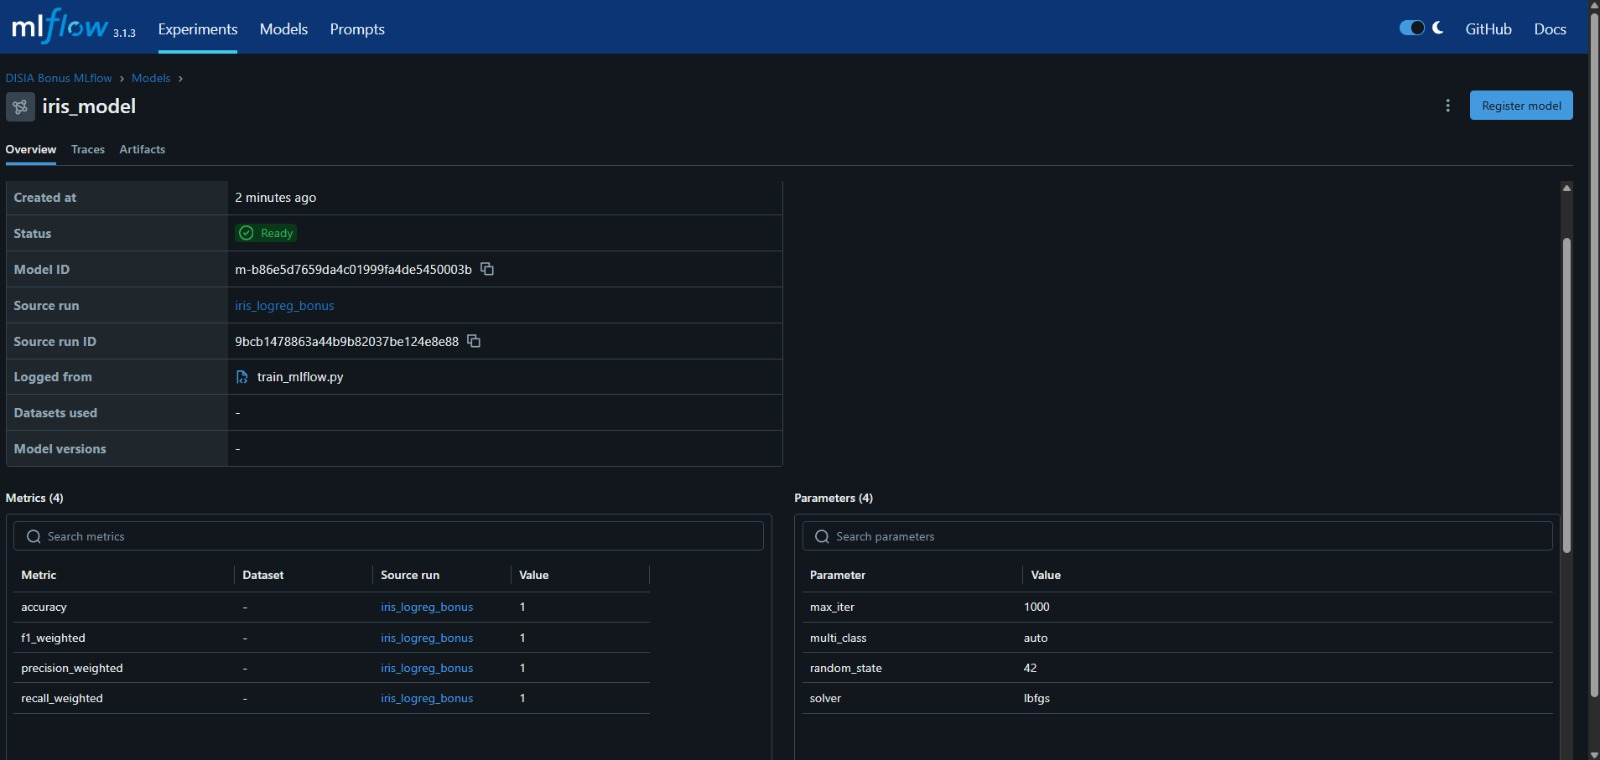
\includegraphics[width=\textwidth]{Pictures/mlflow_experiment.jpg}
    \caption{Vista general del experimento registrado en MLflow.}
    \label{fig:mlflow-experiment}
\end{figure}

La Figura~\ref{fig:mlflow-run} presenta el detalle de la ejecuci\'on, incluyendo m\'etricas, par\'ametros y metadatos
de la run. Esta captura permite comprobar que el entrenamiento no solo se ejecut\'o correctamente, sino que adem\'as qued\'o
documentado con informaci\'on reproducible sobre la configuraci\'on utilizada.

\begin{figure}[htbp]
    \centering
    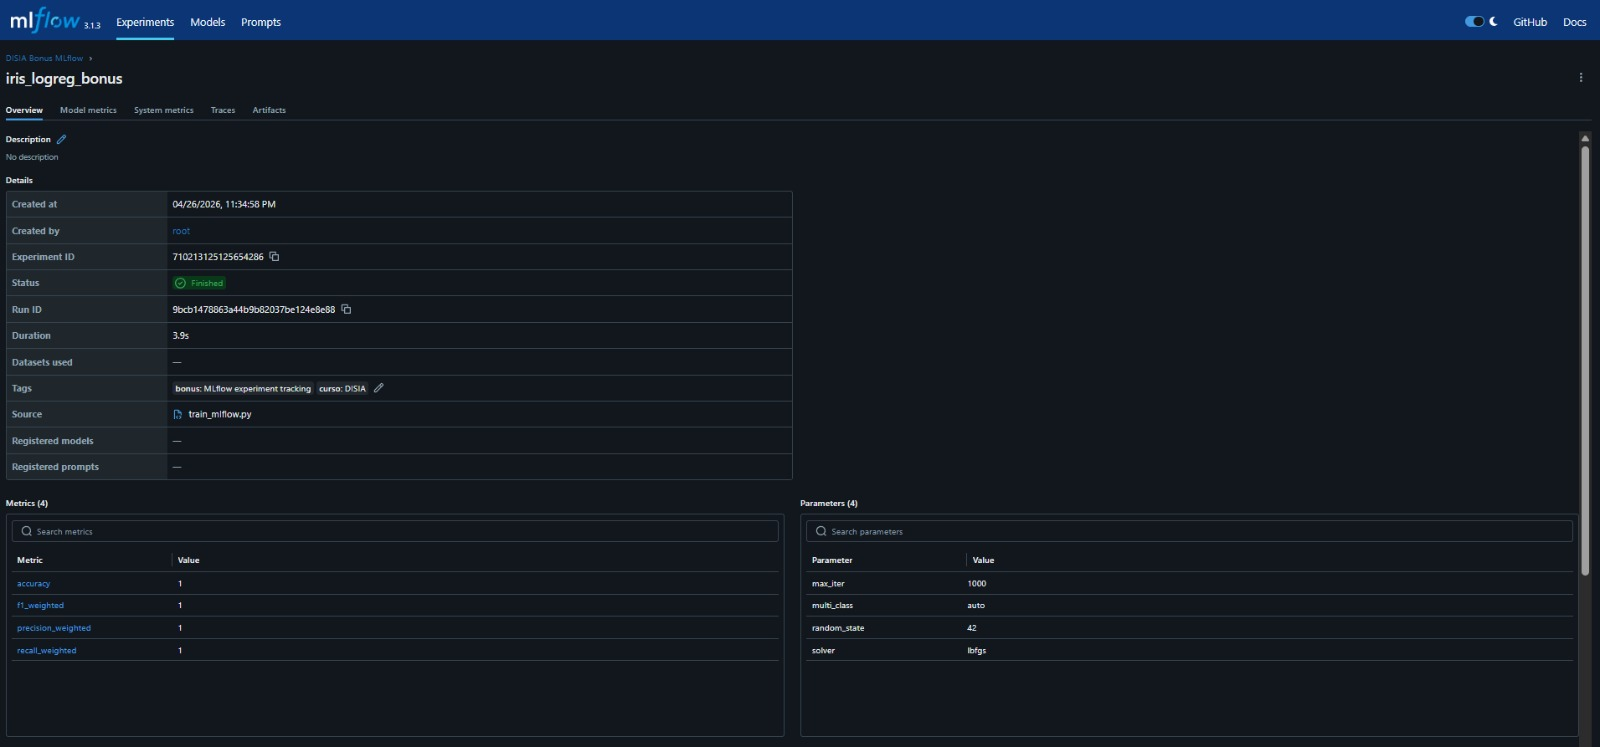
\includegraphics[width=\textwidth]{Pictures/mlflow_run.jpg}
    \caption{Detalle de la ejecuci\'on registrada, incluyendo m\'etricas y par\'ametros.}
    \label{fig:mlflow-run}
\end{figure}

Finalmente, la Figura~\ref{fig:mlflow-model} muestra el modelo almacenado en MLflow y vinculado a la ejecuci\'on de origen.
Esto demuestra que el bonus no se limit\'o al registro de m\'etricas, sino que tambi\'en incluy\'o el almacenamiento del artefacto
del modelo junto con su trazabilidad experimental.

\begin{figure}[htbp]
    \centering
    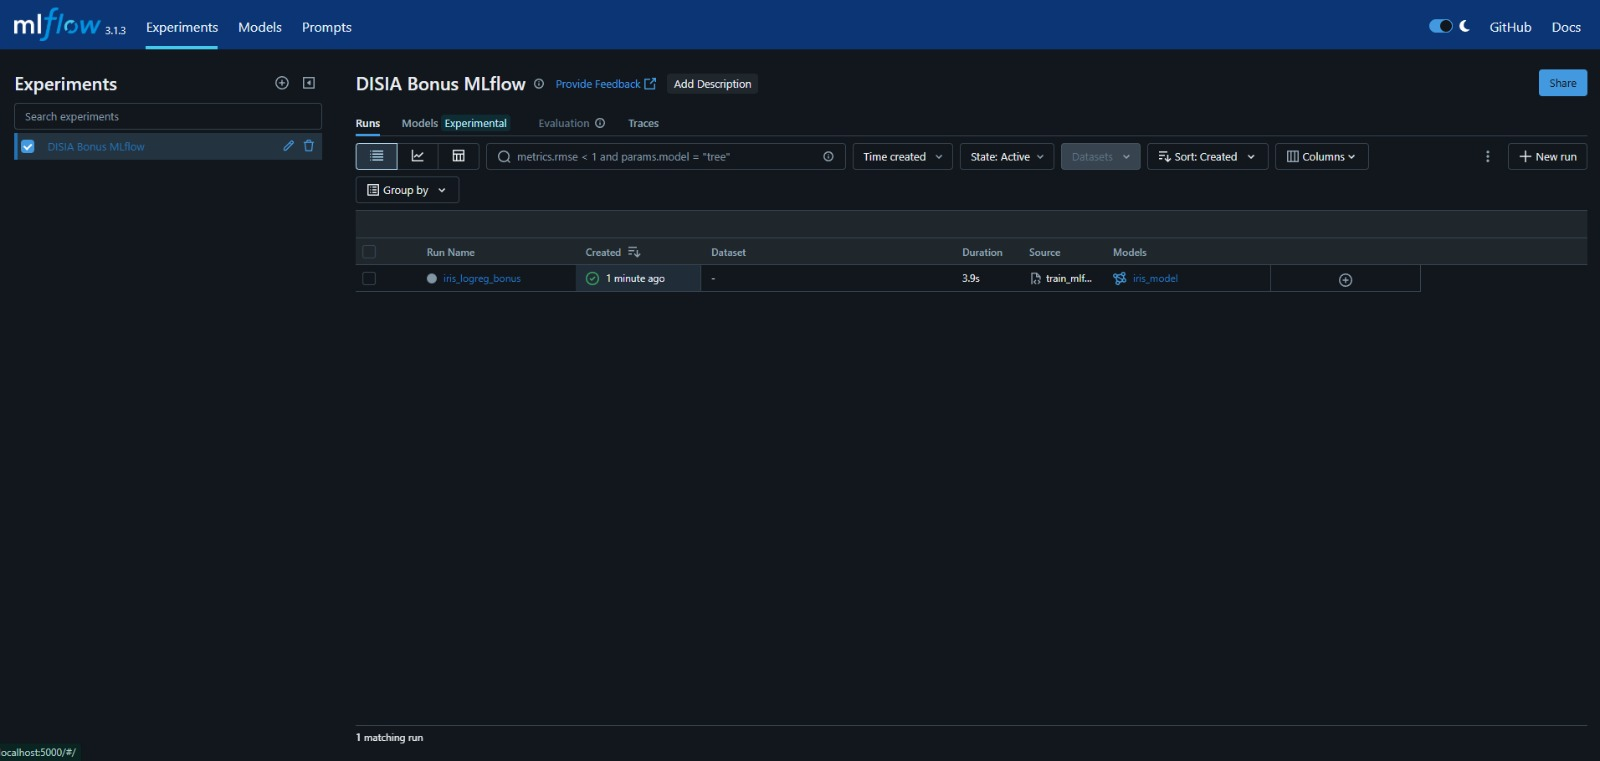
\includegraphics[width=\textwidth]{Pictures/mlflow_model.jpg}
    \caption{Modelo almacenado en MLflow y vinculado a la ejecuci\'on de origen.}
    \label{fig:mlflow-model}
\end{figure}

\section{Valoraci\'on final del hito}

El Hito 4 ha permitido transformar el trabajo previo de modelado en un sistema desplegable y reutilizable. La separaci\'on entre entrenamiento
e inferencia, junto con la contenerizaci\'on del proyecto, mejora la organizaci\'on del c\'odigo y aproxima la soluci\'on a un entorno real de
explotaci\'on.

Adicionalmente, la incorporaci\'on de MLflow como bonus aporta una primera capa de seguimiento experimental propia de flujos MLOps. Aunque se
trata de una implementaci\'on local y acad\'emica, el resultado demuestra la viabilidad de evolucionar el proyecto hacia arquitecturas m\'as
completas de monitorizaci\'on, versionado y despliegue. En conjunto, las decisiones de modularizaci\'on adoptadas han incrementado ligeramente
la complejidad estructural del proyecto, pero a cambio han mejorado su mantenibilidad, su claridad arquitect\'onica y su proximidad a un
escenario real de operaci\'on.